\subsubsection{UC8 - Copia del prompt generato}\label{UC8}

\begin{figure}[H]
  \centering
  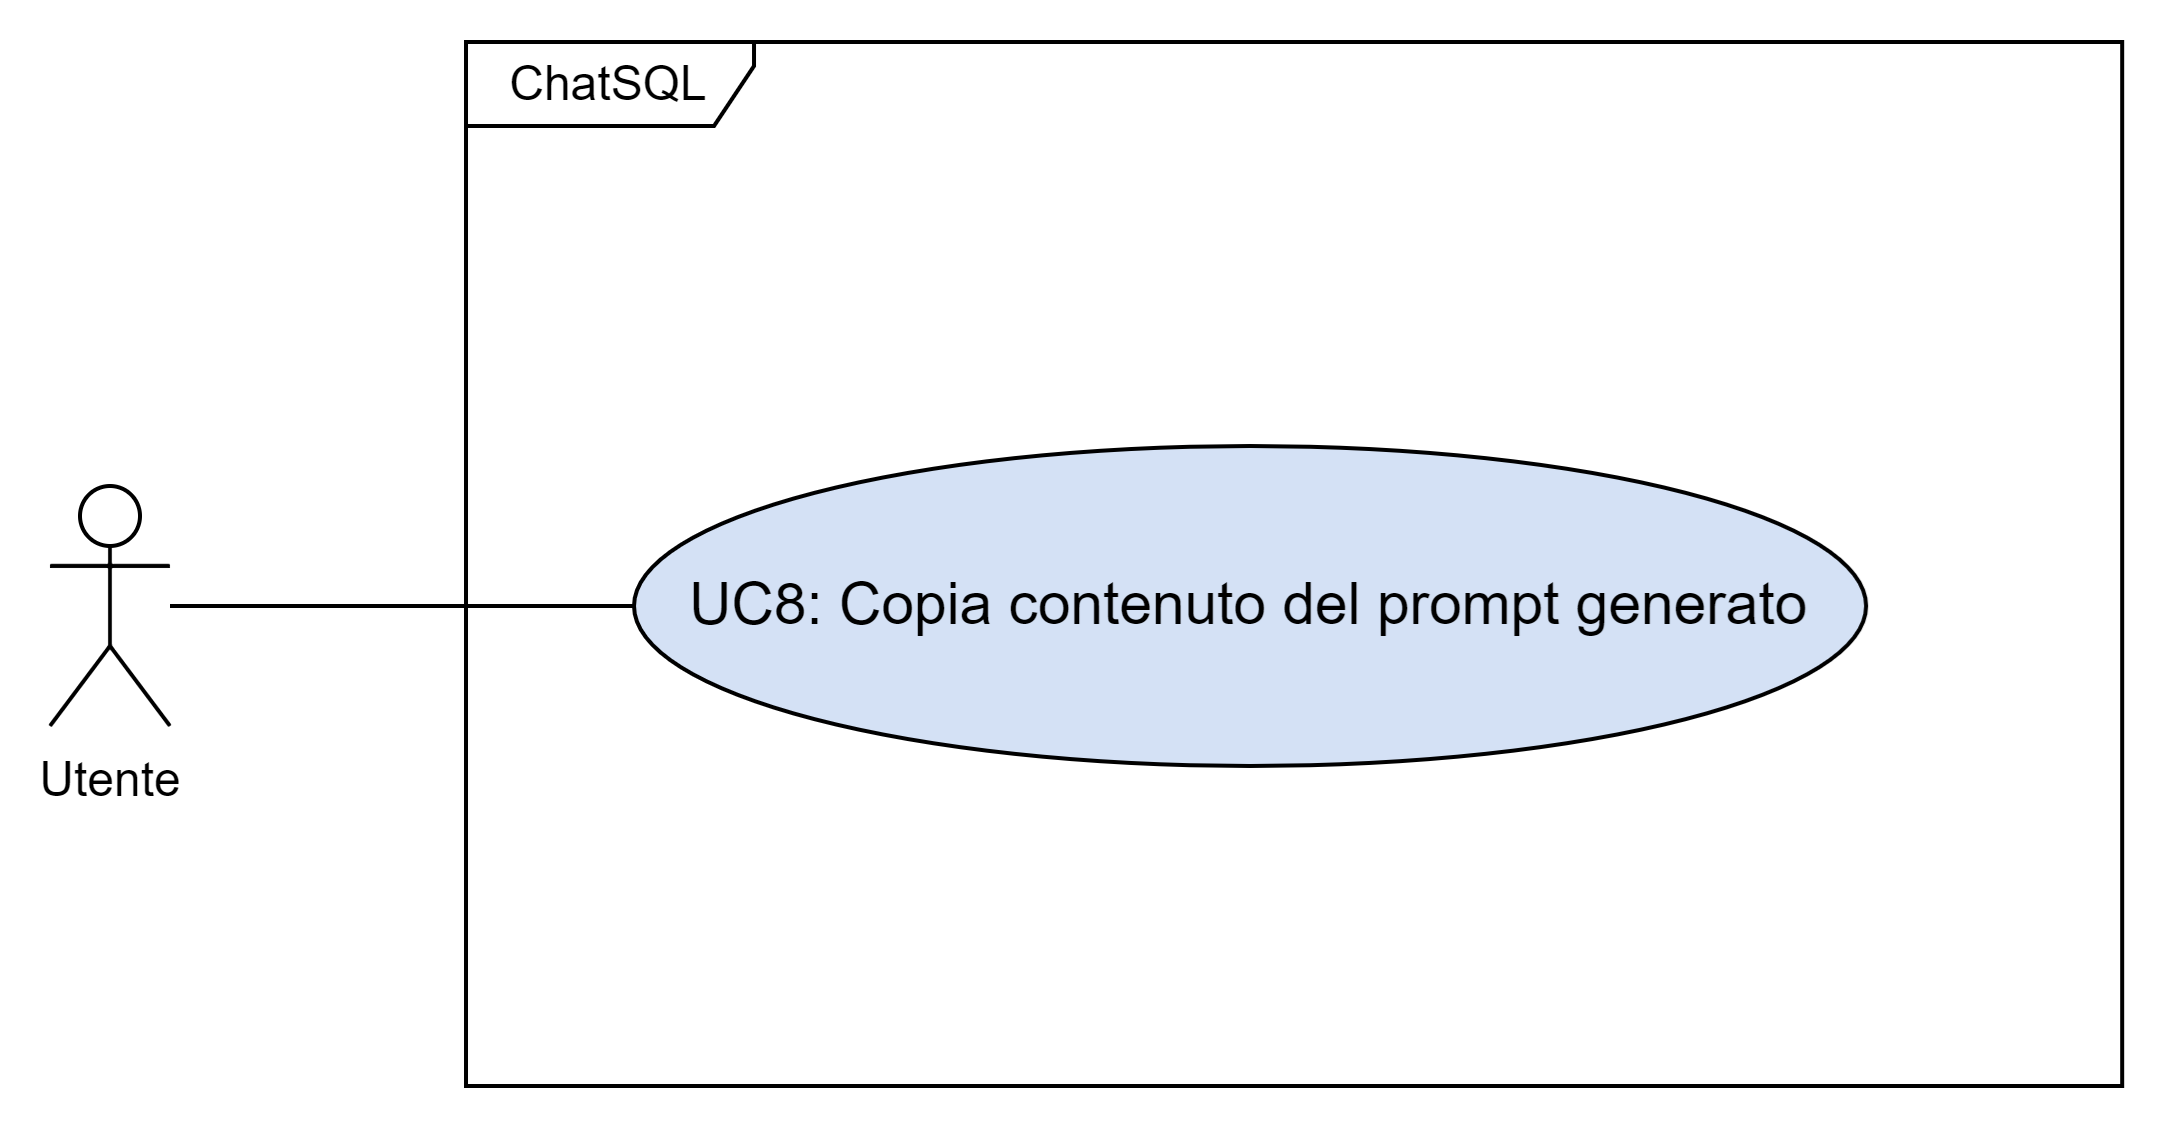
\includegraphics[width=0.90\textwidth]{assets/uc8.png}
  \caption{UC8}
\end{figure}

\paragraph*{Descrizione}
L'Utente può copiare il contenuto del \glossario{prompt} negli appunti di sistema.

\paragraph*{Attori principali}
Utente

\paragraph*{Precondizioni}
\begin{itemize}
  \item L'applicazione è stata avviata con successo;
  \item Il sistema ha generato almeno un \glossario{prompt}.  
\end{itemize}

\paragraph*{Postcondizioni}
\begin{itemize}
  \item Il \glossario{prompt} viene copiato negli appunti di sistema dell'Utente.
\end{itemize}

\paragraph*{Trigger}
L'Utente desidera copiare un \glossario{prompt}, con l'obiettivo di utilizzarlo in un servizio esterno che implementa \glossario{LLM}.

\paragraph*{Scenario principale}
\begin{enumerate}
  \item L'Utente seleziona la funzionalità "Copia";
  \item Negli appunti di sistema viene salvata una copia del prompt.
\end{enumerate}